\unnumberedSection[concept]{Game Concept}

As mentioned before, the concept of the game we are planning to develop is inspired from the vintage video game series called \textit{Bomberman}, first developed in 1983 by Hudson Soft. In those game, the user usually incarnate a robot that try to find its way out of the maze by destroying walls and find the key that will open the door to the next level. \autoref{fig:bombermanGameplay1983} shows this game in action. Multiplayer versions of this game have been developed since 1990, but for a long time remained a side feature of the original singleplayer game. \cite{wiki:bomberman} \\

\begin{figure}[ht]
  \begin{center}
    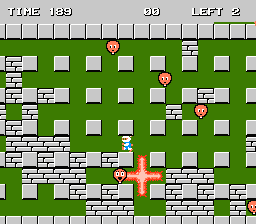
\includegraphics[width=1\textwidth, height=0.4\textheight,keepaspectratio]{Bomberman_(NES)_gameplay}
    \caption{Gameplay of the original Bomberman on NES (1983)}
    \label{fig:bombermanGameplay1983}
  \end{center}
  \vspace{-\baselineskip}
\end{figure}

Even if this game has been commercialized under new official console versions for more than 20 years, we still think that this concept can be pushed forward by the addition of new characters, items, maps, abilities, etc. and by creating a mobile version out of it. Despite this long success story, \textit{Bomberman} series did not see any new version released from 2010 to 2016. Its latest version at the moment is called \textit{Super Bomberman R} and is focusing on the mutliplayer gameplay on a really similar way that we are about to do. \\

In our versions of the game, all the basic elements of the game will be conserved.
\begin{itemize}
  \item 2D maze where the character can only move up, down, right or left
  \item Mix of destructible and indestructible walls
  \item Items dropping off the destroyed walls
\end{itemize}
The new elements added will mostly be related to the special abilities of the each character. Some examples of those abilities are defusing bombs, building walls, summoning \glspl{npc} and kicking bombs. Great care will be needed to balance the cool down of those special abilities to avoid some characters to be over-powered comparatively to the others. Moreover, we are planning to use bigger maps and smaller camera view that will allow us to use more detailed graphics and to add additional difficulty to the game since a given user will not necessarily know what is happening on the rest of the map. \\

We are expecting the gameplay to be fast and to be flexible enough to account for many strategies. Users will be rushed to find the opponents to avoid that they build too much in force. For this part, we are planing to build a skill upgrading system that will introduce some variations depending on the character. Those variations will create some characters that will be stronger in early fights and some others that will only reach their full capacities around the end of the match. Also, the point system will be created in such a way that the only real way to make points will be to tear down the other users whereas breaking walls will only account for small amount of points. These dynamics will necessarily push the opponents to engage the fight faster. \\

Another interesting aspect of the game will be the accumulation of badges according to the way the users are playing the game. Based on the statistics, the different badges will be unlocked. Down here is a short list of achievements that is currently considered to be included in the game.
\begin{multicols}{2}
  \begin{description}[style=nextline]
    \item [Collateral Damage] Kill 3 adversaries at the same time
    \item [Excavator] Destroy 1000 walls
    \item [Kamikaze] Eliminate everybody on the map (including you) and win the match
    \item [Veteran] Play 100 Matches
  \end{description}
\end{multicols}
Furthermore, all the users of the application will be ranked according to their overall statistics. This overall score will have to take several parameters into consideration to favor active users and distinguish skilled users at the same time. \\

Due to the simplicity of the gameplay, some efforts will be necessary in order to attract modern users by using smooth graphics and intuitive \gls{ui}. Some mobile versions of this game have already been created. The \autoref{fig:targetedGameplay} show one of these that we found particularly nice in terms of the graphical interface. We expect ending up with something that looks somewhat similar to this.

\begin{figure}[hb]
  \begin{center}
    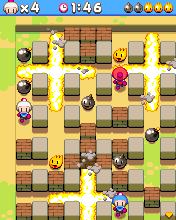
\includegraphics[width=1\textwidth, height=0.375\textheight,keepaspectratio]{bomberman_mobile_by_kennethfejer}
    \caption{Bomberman mobile in action by \href{Kenneth Fejer}{\cite{fejer}}}
    \label{fig:targetedGameplay}
  \end{center}
  \vspace{-\baselineskip}
\end{figure}
